 
\subsection{Experiment setup}

We implement the benchmarks on Google Cloud, which is a mainstream cloud platform to provide serverless functions. 
For local measurements, we use an Ubuntu 20.04-64bit machine with Intel(R) Core(TM) i7-8750H CPU @ 2.20GHz processor and 12GB RAM.


\subsection{Factors impacting context switches in serverless environment}

% TODO

\subsection{Measuring local context switches}

All the previous benchmarks\cite{cs-web,cs-datasize,cs-lmbench,cs-pipes} are implemented in C language.
However, currently Google Cloud only supports functions written in Node.js, Go, Java, Python and Ruby.
Consider that Python is one of the most popular languages, rewriting the prior benchmarks in Python and examining its correctness in local PC is important.

The context switch time measured by the first three benchmarks in local PC is usually among 2us from Table~\ref{tab:experiment1}.
However, when it's rewritten by Python, the measured time is 10 times larger than previous results. 
The reason might be that extra execution is added to the time measurement when translating the language.
What's more, the C programs execute faster as compiled programs while Python executes slower due its interpreted programs.
Therefore, these extra execution time is more obvious when using python. 
We aim to improve the Python version to make the result close to previous benchmarks.

\begin{center}
    \begin{table}
    \begin{tabular}{||c c c c c||} 
     \hline
     Benchmark & Pipe & Condition Var & lmbench & Pipe(python) \\ 
     \hline
     Time(/us) & 1.96 & 2.29 & 1.78 & 33.6\\ 
     \hline
    \end{tabular}
    \caption{\label{tab:experiment1}Context switch time by different benchmarks}
\end{table}
    
\end{center}

\subsection{Measuring context switches in the cloud}



% Figure~\ref{fig:attack-1}.

% \begin{figure}
% 	\centering
% 	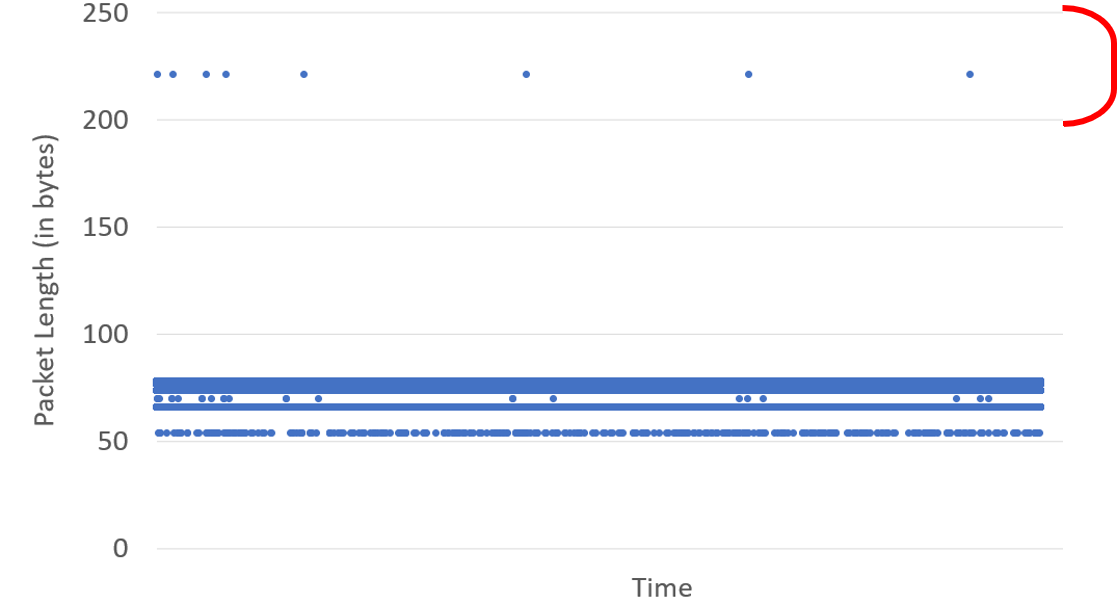
\includegraphics[width=\linewidth]{figure/attack1.png}
% 	\caption{Plot of Modbus packet lengths}
% 	\label{fig:attack-1}
% \end{figure}
